% Options for packages loaded elsewhere
% Options for packages loaded elsewhere
\PassOptionsToPackage{unicode}{hyperref}
\PassOptionsToPackage{hyphens}{url}
\PassOptionsToPackage{dvipsnames,svgnames,x11names}{xcolor}
%
\documentclass[
  letterpaper,
  DIV=11,
  numbers=noendperiod]{scrartcl}
\usepackage{xcolor}
\usepackage{amsmath,amssymb}
\setcounter{secnumdepth}{-\maxdimen} % remove section numbering
\usepackage{iftex}
\ifPDFTeX
  \usepackage[T1]{fontenc}
  \usepackage[utf8]{inputenc}
  \usepackage{textcomp} % provide euro and other symbols
\else % if luatex or xetex
  \usepackage{unicode-math} % this also loads fontspec
  \defaultfontfeatures{Scale=MatchLowercase}
  \defaultfontfeatures[\rmfamily]{Ligatures=TeX,Scale=1}
\fi
\usepackage{lmodern}
\ifPDFTeX\else
  % xetex/luatex font selection
\fi
% Use upquote if available, for straight quotes in verbatim environments
\IfFileExists{upquote.sty}{\usepackage{upquote}}{}
\IfFileExists{microtype.sty}{% use microtype if available
  \usepackage[]{microtype}
  \UseMicrotypeSet[protrusion]{basicmath} % disable protrusion for tt fonts
}{}
\makeatletter
\@ifundefined{KOMAClassName}{% if non-KOMA class
  \IfFileExists{parskip.sty}{%
    \usepackage{parskip}
  }{% else
    \setlength{\parindent}{0pt}
    \setlength{\parskip}{6pt plus 2pt minus 1pt}}
}{% if KOMA class
  \KOMAoptions{parskip=half}}
\makeatother
% Make \paragraph and \subparagraph free-standing
\makeatletter
\ifx\paragraph\undefined\else
  \let\oldparagraph\paragraph
  \renewcommand{\paragraph}{
    \@ifstar
      \xxxParagraphStar
      \xxxParagraphNoStar
  }
  \newcommand{\xxxParagraphStar}[1]{\oldparagraph*{#1}\mbox{}}
  \newcommand{\xxxParagraphNoStar}[1]{\oldparagraph{#1}\mbox{}}
\fi
\ifx\subparagraph\undefined\else
  \let\oldsubparagraph\subparagraph
  \renewcommand{\subparagraph}{
    \@ifstar
      \xxxSubParagraphStar
      \xxxSubParagraphNoStar
  }
  \newcommand{\xxxSubParagraphStar}[1]{\oldsubparagraph*{#1}\mbox{}}
  \newcommand{\xxxSubParagraphNoStar}[1]{\oldsubparagraph{#1}\mbox{}}
\fi
\makeatother


\usepackage{longtable,booktabs,array}
\newcounter{none} % for unnumbered tables
\usepackage{calc} % for calculating minipage widths
% Correct order of tables after \paragraph or \subparagraph
\usepackage{etoolbox}
\makeatletter
\patchcmd\longtable{\par}{\if@noskipsec\mbox{}\fi\par}{}{}
\makeatother
% Allow footnotes in longtable head/foot
\IfFileExists{footnotehyper.sty}{\usepackage{footnotehyper}}{\usepackage{footnote}}
\makesavenoteenv{longtable}
\usepackage{graphicx}
\makeatletter
\newsavebox\pandoc@box
\newcommand*\pandocbounded[1]{% scales image to fit in text height/width
  \sbox\pandoc@box{#1}%
  \Gscale@div\@tempa{\textheight}{\dimexpr\ht\pandoc@box+\dp\pandoc@box\relax}%
  \Gscale@div\@tempb{\linewidth}{\wd\pandoc@box}%
  \ifdim\@tempb\p@<\@tempa\p@\let\@tempa\@tempb\fi% select the smaller of both
  \ifdim\@tempa\p@<\p@\scalebox{\@tempa}{\usebox\pandoc@box}%
  \else\usebox{\pandoc@box}%
  \fi%
}
% Set default figure placement to htbp
\def\fps@figure{htbp}
\makeatother


% definitions for citeproc citations
\NewDocumentCommand\citeproctext{}{}
\NewDocumentCommand\citeproc{mm}{%
  \begingroup\def\citeproctext{#2}\cite{#1}\endgroup}
\makeatletter
 % allow citations to break across lines
 \let\@cite@ofmt\@firstofone
 % avoid brackets around text for \cite:
 \def\@biblabel#1{}
 \def\@cite#1#2{{#1\if@tempswa , #2\fi}}
\makeatother
\newlength{\cslhangindent}
\setlength{\cslhangindent}{1.5em}
\newlength{\csllabelwidth}
\setlength{\csllabelwidth}{3em}
\newenvironment{CSLReferences}[2] % #1 hanging-indent, #2 entry-spacing
 {\begin{list}{}{%
  \setlength{\itemindent}{0pt}
  \setlength{\leftmargin}{0pt}
  \setlength{\parsep}{0pt}
  % turn on hanging indent if param 1 is 1
  \ifodd #1
   \setlength{\leftmargin}{\cslhangindent}
   \setlength{\itemindent}{-1\cslhangindent}
  \fi
  % set entry spacing
  \setlength{\itemsep}{#2\baselineskip}}}
 {\end{list}}
\usepackage{calc}
\newcommand{\CSLBlock}[1]{\hfill\break\parbox[t]{\linewidth}{\strut\ignorespaces#1\strut}}
\newcommand{\CSLLeftMargin}[1]{\parbox[t]{\csllabelwidth}{\strut#1\strut}}
\newcommand{\CSLRightInline}[1]{\parbox[t]{\linewidth - \csllabelwidth}{\strut#1\strut}}
\newcommand{\CSLIndent}[1]{\hspace{\cslhangindent}#1}



\setlength{\emergencystretch}{3em} % prevent overfull lines

\providecommand{\tightlist}{%
  \setlength{\itemsep}{0pt}\setlength{\parskip}{0pt}}



 


\usepackage{fvextra}
\usepackage{float}
\DefineVerbatimEnvironment{Highlighting}{Verbatim}{breaklines,breakanywhere,commandchars=\\\{\}}
\KOMAoption{captions}{tableheading}
\makeatletter
\@ifpackageloaded{caption}{}{\usepackage{caption}}
\AtBeginDocument{%
\ifdefined\contentsname
  \renewcommand*\contentsname{Table of contents}
\else
  \newcommand\contentsname{Table of contents}
\fi
\ifdefined\listfigurename
  \renewcommand*\listfigurename{List of Figures}
\else
  \newcommand\listfigurename{List of Figures}
\fi
\ifdefined\listtablename
  \renewcommand*\listtablename{List of Tables}
\else
  \newcommand\listtablename{List of Tables}
\fi
\ifdefined\figurename
  \renewcommand*\figurename{Figure}
\else
  \newcommand\figurename{Figure}
\fi
\ifdefined\tablename
  \renewcommand*\tablename{Table}
\else
  \newcommand\tablename{Table}
\fi
}
\@ifpackageloaded{float}{}{\usepackage{float}}
\floatstyle{ruled}
\@ifundefined{c@chapter}{\newfloat{codelisting}{h}{lop}}{\newfloat{codelisting}{h}{lop}[chapter]}
\floatname{codelisting}{Listing}
\newcommand*\listoflistings{\listof{codelisting}{List of Listings}}
\makeatother
\makeatletter
\makeatother
\makeatletter
\@ifpackageloaded{caption}{}{\usepackage{caption}}
\@ifpackageloaded{subcaption}{}{\usepackage{subcaption}}
\makeatother
\usepackage{bookmark}
\IfFileExists{xurl.sty}{\usepackage{xurl}}{} % add URL line breaks if available
\urlstyle{same}
\hypersetup{
  pdftitle={Dissolved Oxygen Patterns Across NCOS Sites},
  pdfauthor={Phoebe Dupa, Rebecca Martinez, and Shucan Zhao},
  colorlinks=true,
  linkcolor={blue},
  filecolor={Maroon},
  citecolor={Blue},
  urlcolor={Blue},
  pdfcreator={LaTeX via pandoc}}


\title{Dissolved Oxygen Patterns Across NCOS Sites}
\author{Phoebe Dupa, Rebecca Martinez, and Shucan Zhao}
\date{10 June 2026}
\begin{document}
\maketitle

\renewcommand*\contentsname{Table of contents}
{
\setcounter{tocdepth}{3}
\tableofcontents
}

\section{Introduction}\label{introduction}

North Campus Open Space (NCOS) is a restored wetland connected to the
Devereux Slough system in Goleta, California. The site includes several
channels, bridges, and wetland areas, so water quality may differ across
the system. The North Campus Open Space Restoration Project Monitoring
Report provides background on restoration progress and monitoring at the
site (Rickard 2024). At a restored wetland like NCOS, water quality
monitoring helps show how conditions vary across different parts of the
system.

Dissolved oxygen is a useful water quality measurement because it shows
how much oxygen is available in the water for aquatic organisms. In
shallow wetlands and estuaries, dissolved oxygen can vary by location,
season, time of day, and depth in the water column. These patterns can
be influenced by water movement, temperature, salinity, vegetation,
photosynthesis, respiration, and decomposition (Gale et al. 2006, Nezlin
et al. 2009). These oxygen conditions are also tied to habitat quality.
Low dissolved oxygen can reduce the suitability of wetland and marsh
habitats for fish and other nekton (Smith and Able 2003, Clark et al.
2025). Low oxygen near the bottom of shallow wetlands can also affect
decomposition and invertebrate in the water column (Lee et al. 2017).
For these reasons, dissolved oxygen can be used as an indicator of water
quality and aquatic habitat conditions.

Research from other wetland and estuary systems helps explain why both
site and depth are important to examine. In the Carmel River Lagoon, a
Central California bar-built estuary, dissolved oxygen varied across
different branches of the lagoon as mouth state and hydrologic
conditions changed (Dawson et al. 2023). That pattern is relevant to
NCOS because East Channel, Phelps Bridge, and Venoco Bridge are
different locations within the same coastal wetland system. Other
studies show that shallow lagoons and estuaries can develop vertical
differences in dissolved oxygen when mixing is limited. Under these
conditions, bottom water can become oxygen-depleted while surface water
remains more oxygenated (Gale et al. 2006, Nezlin et al. 2009).
Together, these studies provide a basis for looking at both site-level
differences and vertical differences in dissolved oxygen at NCOS.

The analysis focuses on three NCOS sites: East Channel, Phelps Bridge,
and Venoco Bridge. These sites represent different parts of the wetland
and may differ in water movement, depth, vegetation, salinity, and
connection to other parts of the slough. Within each site, elevation
code is used to examine possible DO stratification, where codes 0, 1,
and 2 correspond to bottom, middle, and upper measurements,
respectively.

This study asks two main questions:

\begin{enumerate}
\def\labelenumi{\arabic{enumi}.}
\tightlist
\item
  How does dissolved oxygen differ across East Channel, Phelps Bridge,
  and Venoco Bridge?
\item
  How does dissolved oxygen stratification differ across elevation-code
  measurement positions within each site?
\end{enumerate}

\section{Methods}\label{methods}

This analysis used NCOS water quality monitoring data from the 2024 and
2025 water years. Sampling was conducted on a regular schedule
throughout the 2024 and 2025 water years. Each site was sampled
approximately weekly, so that dissolved oxygen at each site is
represented by many measurements across both wet and dry seasons. The
analysis focused on three main sites: East Channel, Phelps Bridge, and
Venoco Bridge. These sites were selected because they represent
different parts of the wetland system and had enough dissolved oxygen
measurements to compare. The North Campus Open Space Restoration Project
Monitoring Report provides background on the restoration project and
monitoring at the site (Rickard 2024).

The analysis used NCOS water quality monitoring metadata and YSI water
quality measurements. The metadata included survey information such as
site name, monitoring date, weather notes, water year, and location
information. The YSI dataset included water quality measurements such as
dissolved oxygen, temperature, salinity, conductivity, and elevation
code. NOAA weather data were also available and provided temporal
context for the monitoring dates.

The metadata and YSI water quality data were cleaned and joined so that
each dissolved oxygen measurement was connected to the correct site,
date, water year, and elevation-code position. The final dissolved
oxygen dataset was filtered to include East Channel, Phelps Bridge, and
Venoco Bridge during the 2024 and 2025 water years. The dataset was also
filtered to elevation codes 0, 1, and 2, which represented bottom,
middle, and upper measurements, respectively.

Dissolved oxygen, measured in milligrams per liter, was the main
response variable. Site was used to compare dissolved oxygen across the
three NCOS locations, and elevation code was used to compare dissolved
oxygen across bottom, middle, and upper measurement positions within
each site. Descriptive statistics were calculated before statistical
testing. Dissolved oxygen was summarized by site and by
site/elevation-code combinations using mean, median, first quartile,
third quartile, standard deviation, variance, and sample size.
Stratification difference was also calculated for each site as upper
median dissolved oxygen minus bottom median dissolved oxygen. Positive
values indicated that median dissolved oxygen was higher at the upper
measurement position than at the bottom measurement position.

Figures were created to show dissolved oxygen across sites, dissolved
oxygen across elevation codes within each site, median dissolved oxygen
elevation profiles, and median dissolved oxygen through time by
elevation code and site. Kruskal-Wallis tests were used to compare
dissolved oxygen across groups. For the first question, a Kruskal-Wallis
test compared dissolved oxygen across East Channel, Phelps Bridge, and
Venoco Bridge. When that result was significant, Dunn's post-hoc tests
were used to compare site pairs. For the stratification question,
separate Kruskal-Wallis tests were run within each site to compare
dissolved oxygen across elevation codes. When a within-site result was
significant, Dunn's post-hoc tests were used to compare elevation-code
pairs. Effect sizes were also calculated to describe the strength of the
patterns.

The dataset included repeated monitoring observations across sampling
dates rather than continuous dissolved oxygen sensor measurements. As a
result, the analysis shows patterns across sites, elevation codes, and
sampling dates, but it does not capture all short-term changes that may
happen within a day.

\section{Results}\label{results}

Dissolved oxygen differed across the three NCOS sites. East Channel had
a mean dissolved oxygen value of 7.22 mg/L and a median of 7.28 mg/L.
Phelps Bridge had a mean of 4.30 mg/L and a median of 3.70 mg/L. Venoco
Bridge had a mean of 5.68 mg/L and a median of 5.98 mg/L. The middle
50\% of dissolved oxygen values ranged from 5.44 to 9.65 mg/L at East
Channel, 2.56 to 5.96 mg/L at Phelps Bridge, and 2.29 to 8.35 mg/L at
Venoco Bridge.

\begin{figure}[H]

\centering{

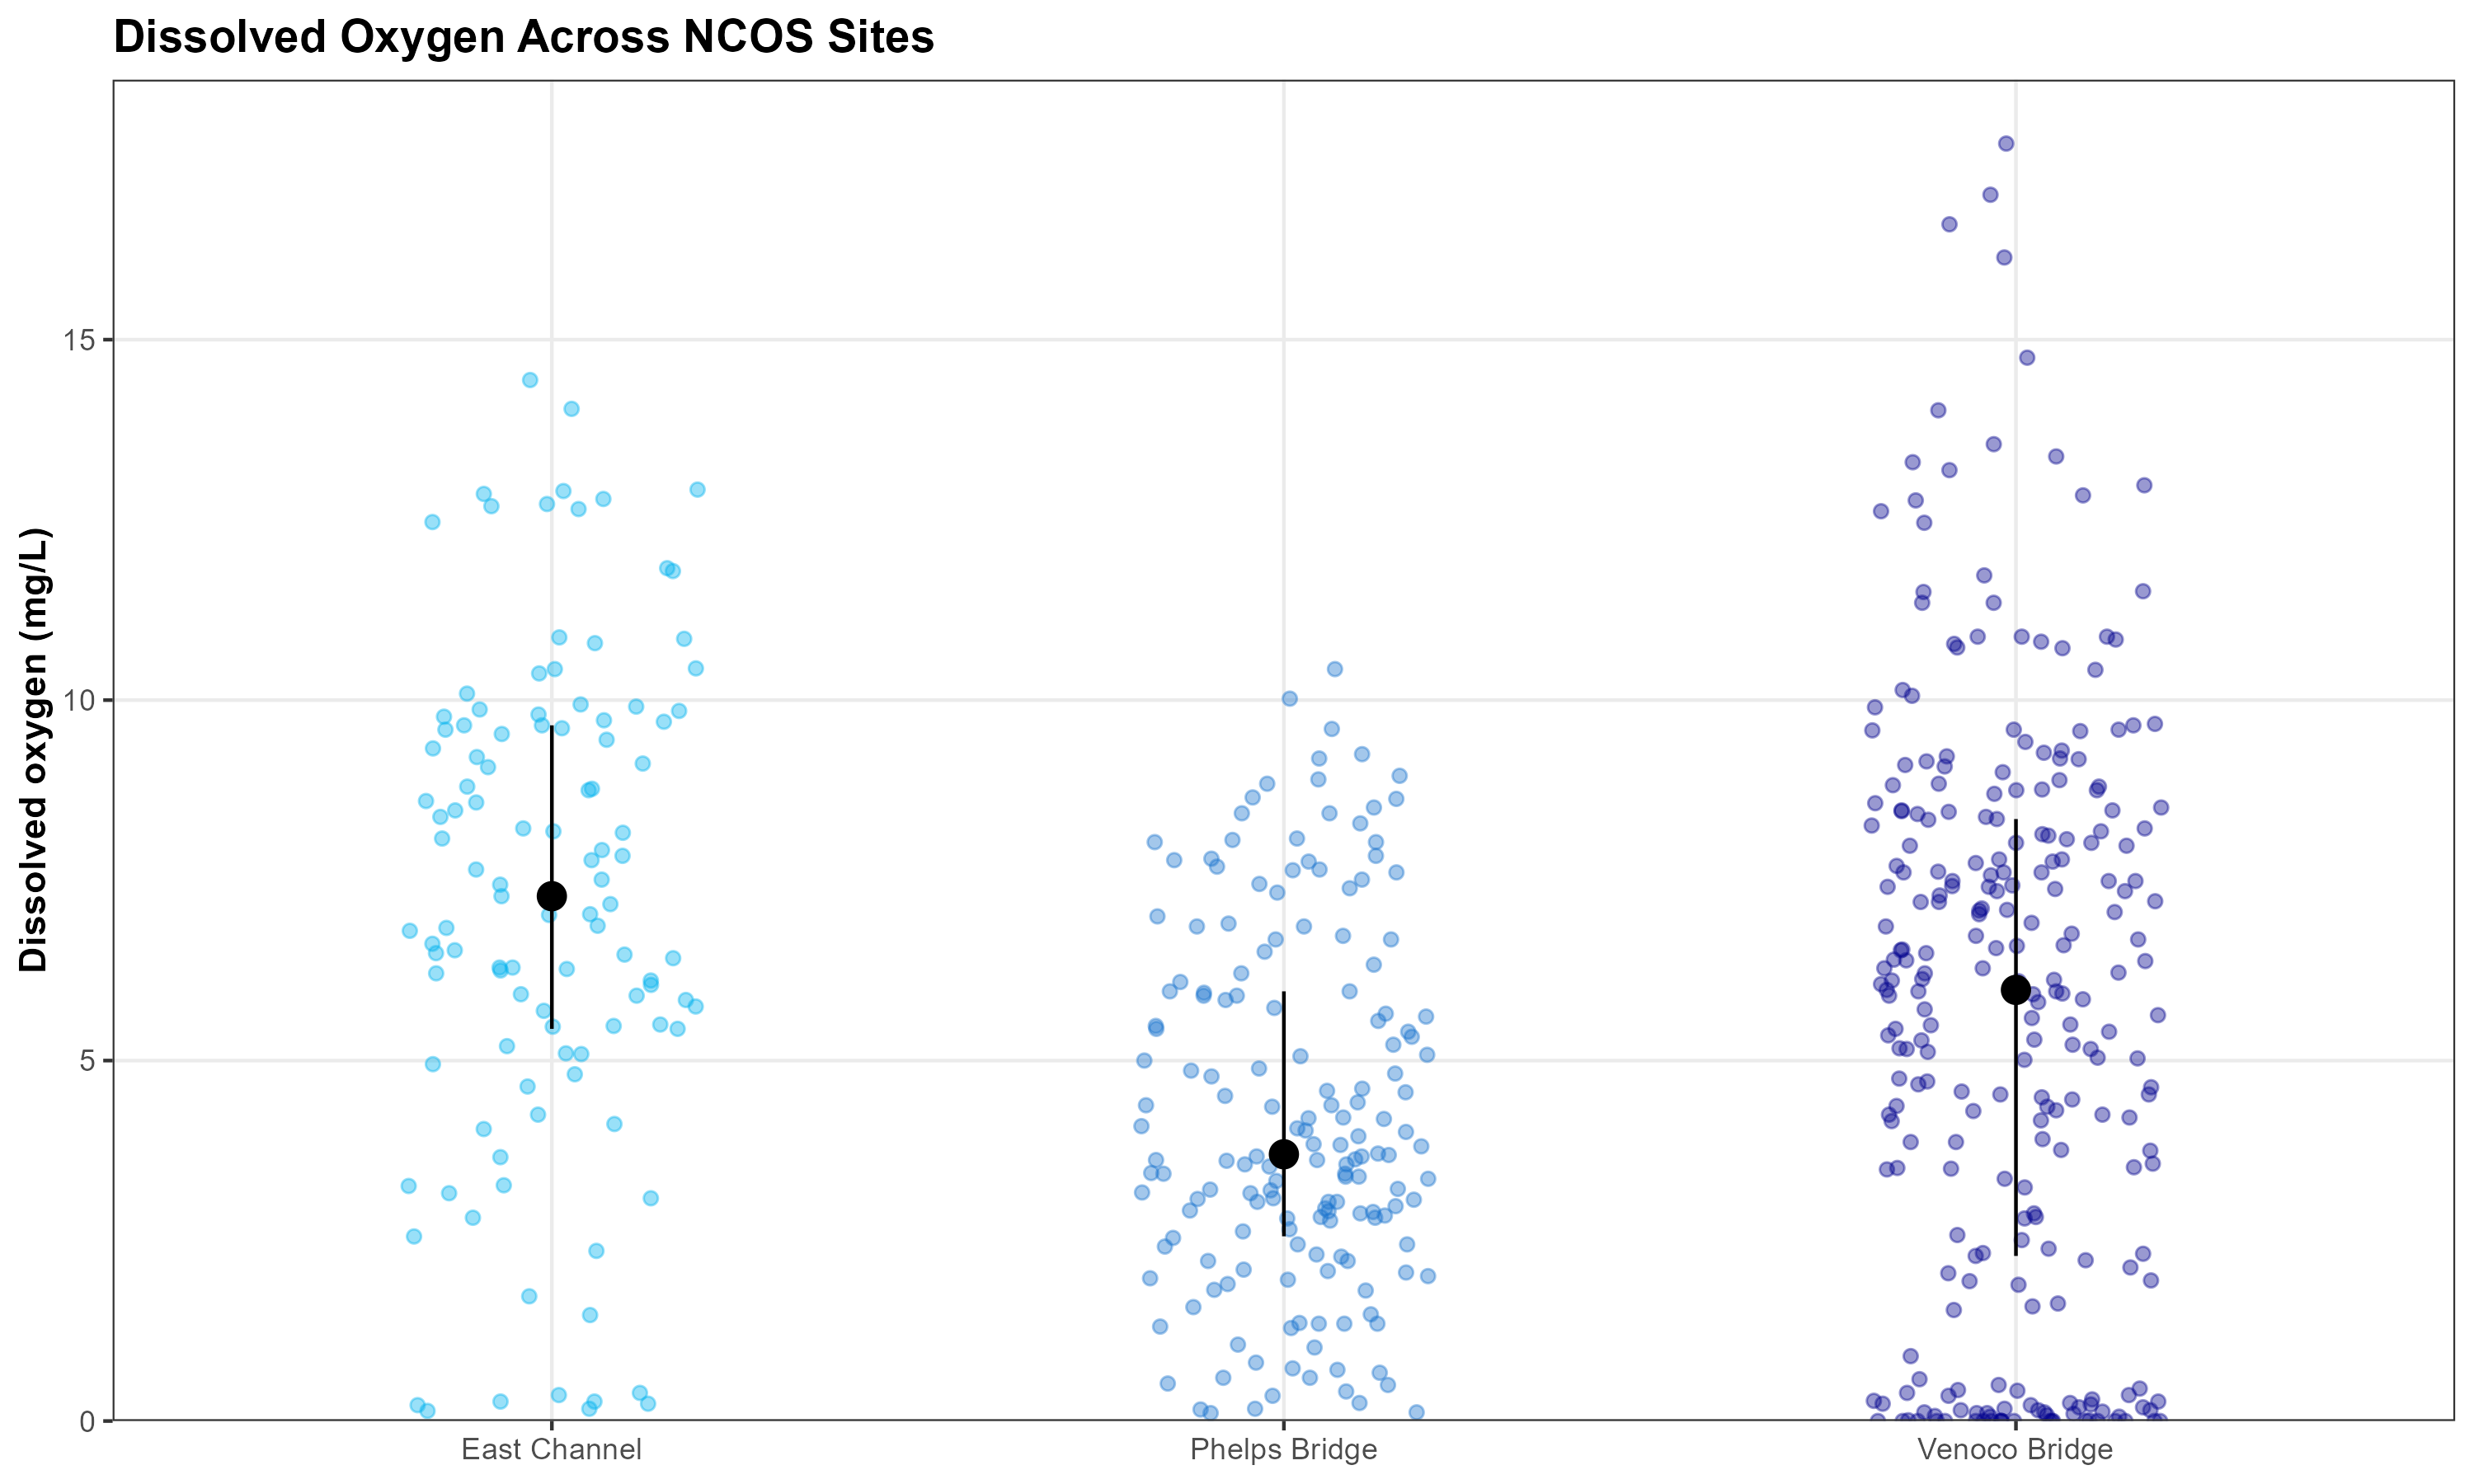
\includegraphics[width=0.85\linewidth,height=\textheight,keepaspectratio]{../images/do_across_sites.png}

}

\caption{\label{fig-do-across-sites}Dissolved oxygen across East
Channel, Phelps Bridge, and Venoco Bridge. Individual points represent
dissolved oxygen observations. Larger black points represent site
medians, and vertical ranges show the first to third quartile range.}

\end{figure}%

Figure~\ref{fig-do-across-sites} presents dissolved oxygen values across
East Channel, Phelps Bridge, and Venoco Bridge. East Channel had the
highest median dissolved oxygen, Phelps Bridge had the lowest median
dissolved oxygen, and Venoco Bridge had the widest spread of values.

A Kruskal-Wallis test showed a significant difference in dissolved
oxygen across sites, \(\chi^2\) = 45.67, df = 2, p \textless{} 0.001.
Dunn's post-hoc tests showed that all three site pairs were
significantly different after adjustment: East Channel and Phelps
Bridge, East Channel and Venoco Bridge, and Phelps Bridge and Venoco
Bridge. The effect size for the site comparison was \(\eta^2_H\) =
0.083, which was classified as moderate.

Median dissolved oxygen values also varied across elevation-code
positions within each site. At East Channel, median dissolved oxygen was
6.66 mg/L at the bottom, 7.96 mg/L in the middle, and 7.17 mg/L at the
upper position. At Phelps Bridge, median dissolved oxygen was 4.14 mg/L
at the bottom, 3.63 mg/L in the middle, and 2.01 mg/L at the upper
position. At Venoco Bridge, median dissolved oxygen was 4.31 mg/L at the
bottom, 6.38 mg/L in the middle, and 7.62 mg/L at the upper position.

\begin{figure}[H]

\centering{

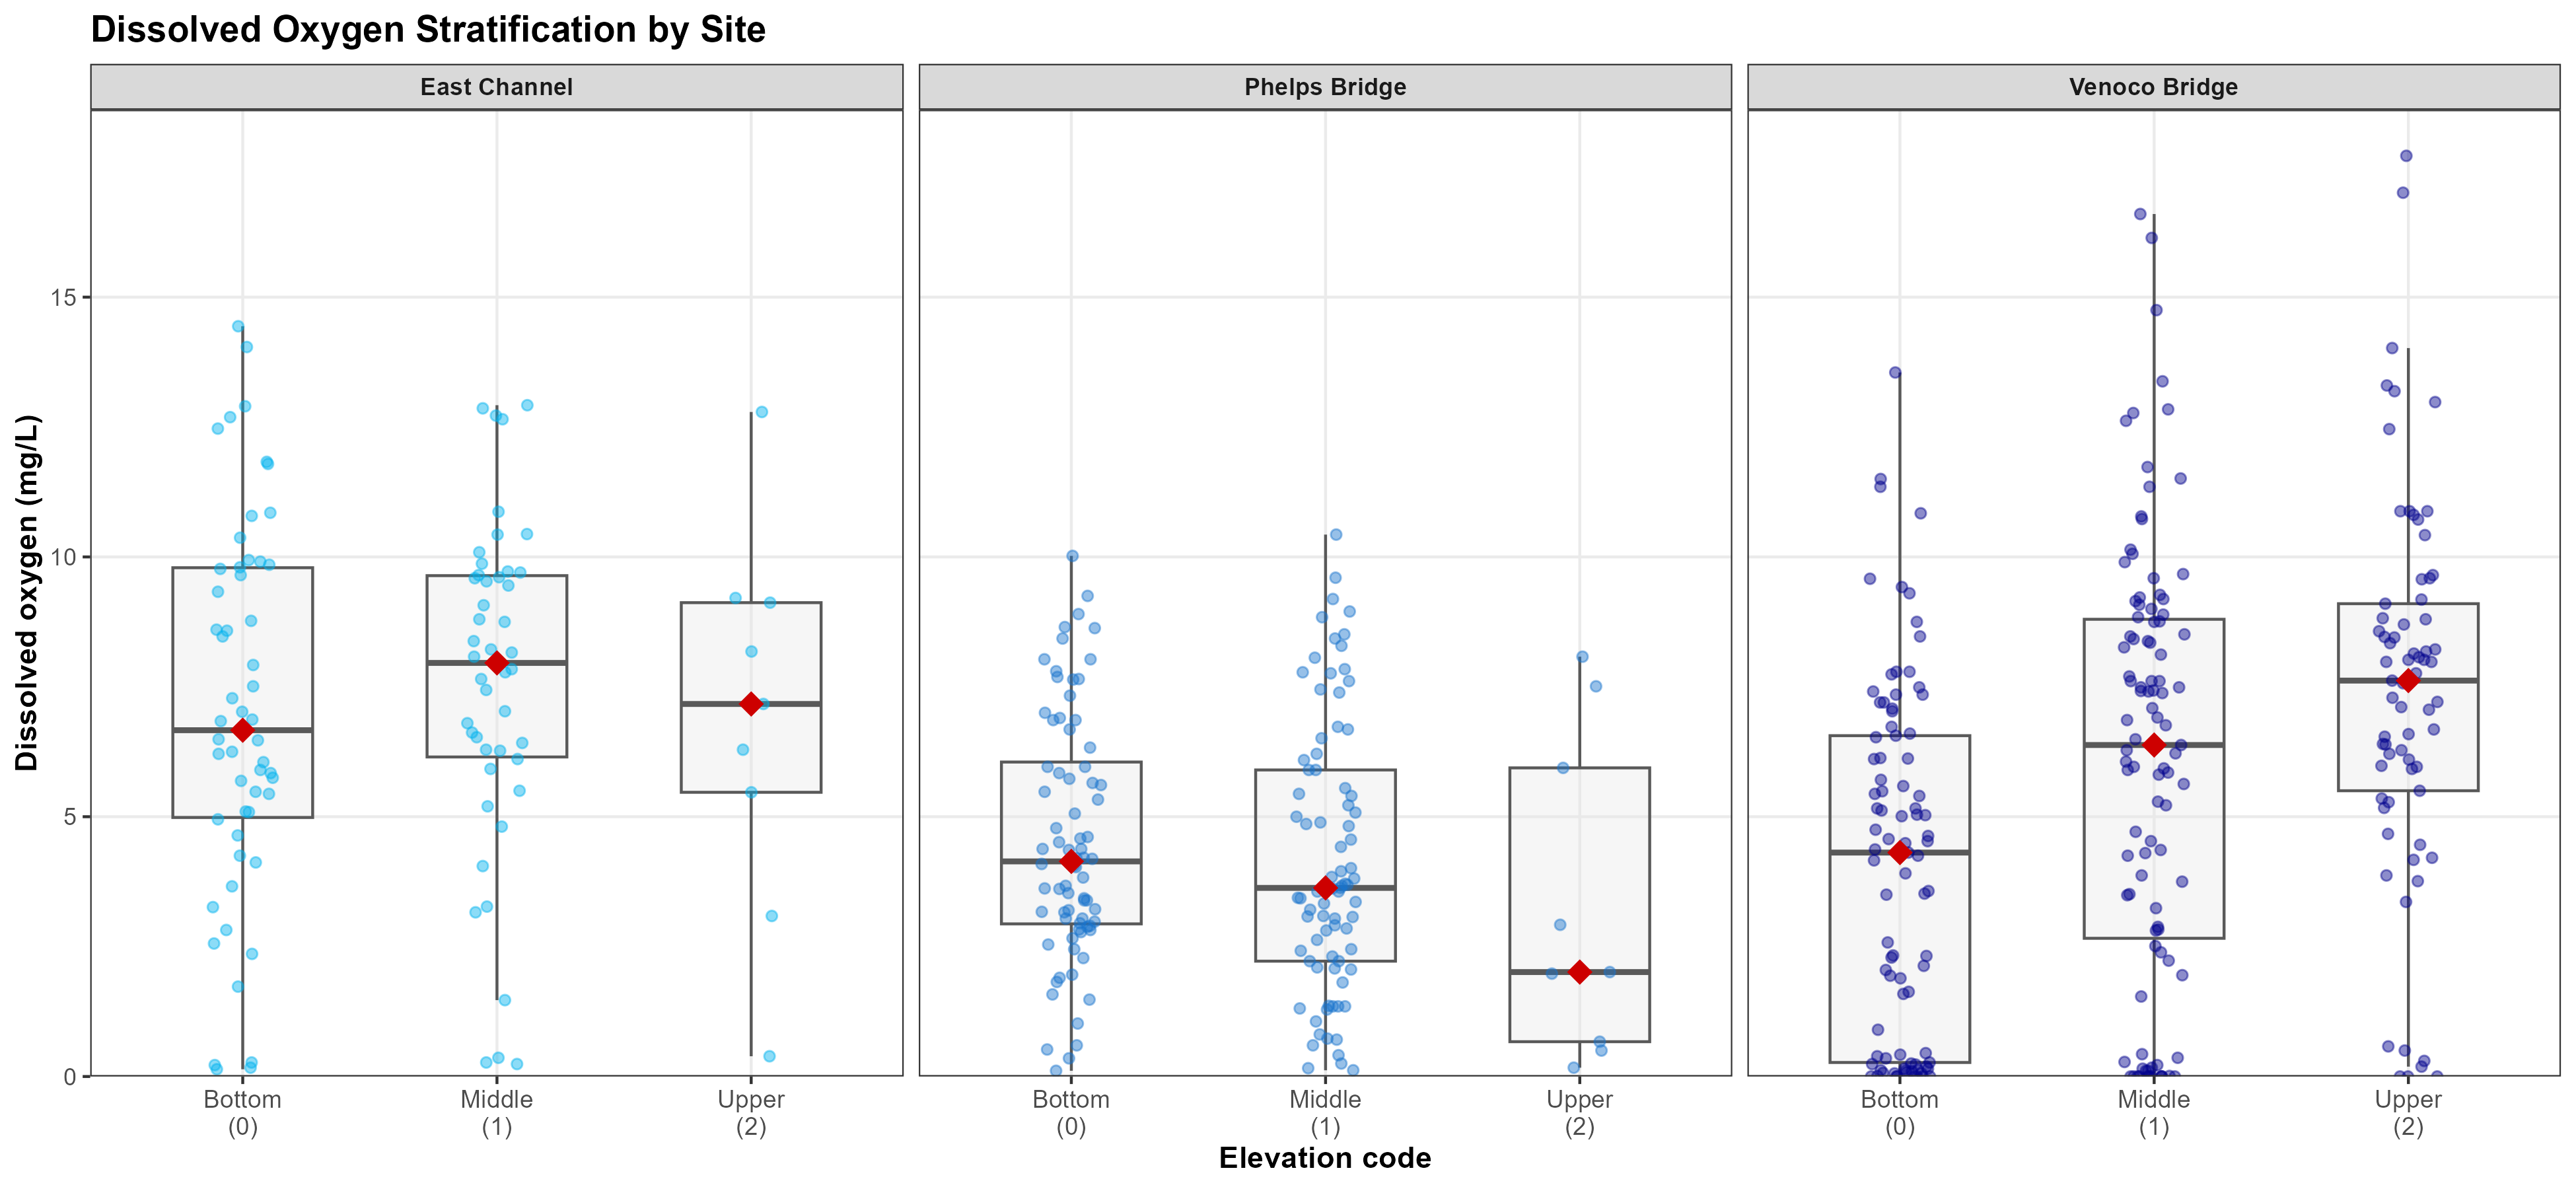
\includegraphics[width=1\linewidth,height=\textheight,keepaspectratio]{../images/do_stratification_by_site.png}

}

\caption{\label{fig-do-stratification}Dissolved oxygen across bottom,
middle, and upper elevation-code positions within each site. Boxplots
show dissolved oxygen distributions, points show individual
observations, and red diamonds show median values.}

\end{figure}%

Figure~\ref{fig-do-stratification} presents the distribution of
dissolved oxygen values by elevation code within each site. The figure
shows the clearest separation among elevation-code positions at Venoco
Bridge.

Stratification difference was calculated as upper median dissolved
oxygen minus bottom median dissolved oxygen. East Channel had a
stratification difference of 0.50 mg/L. Phelps Bridge had a
stratification difference of -2.13 mg/L. Venoco Bridge had a
stratification difference of 3.31 mg/L.

\begin{figure}[H]

\centering{

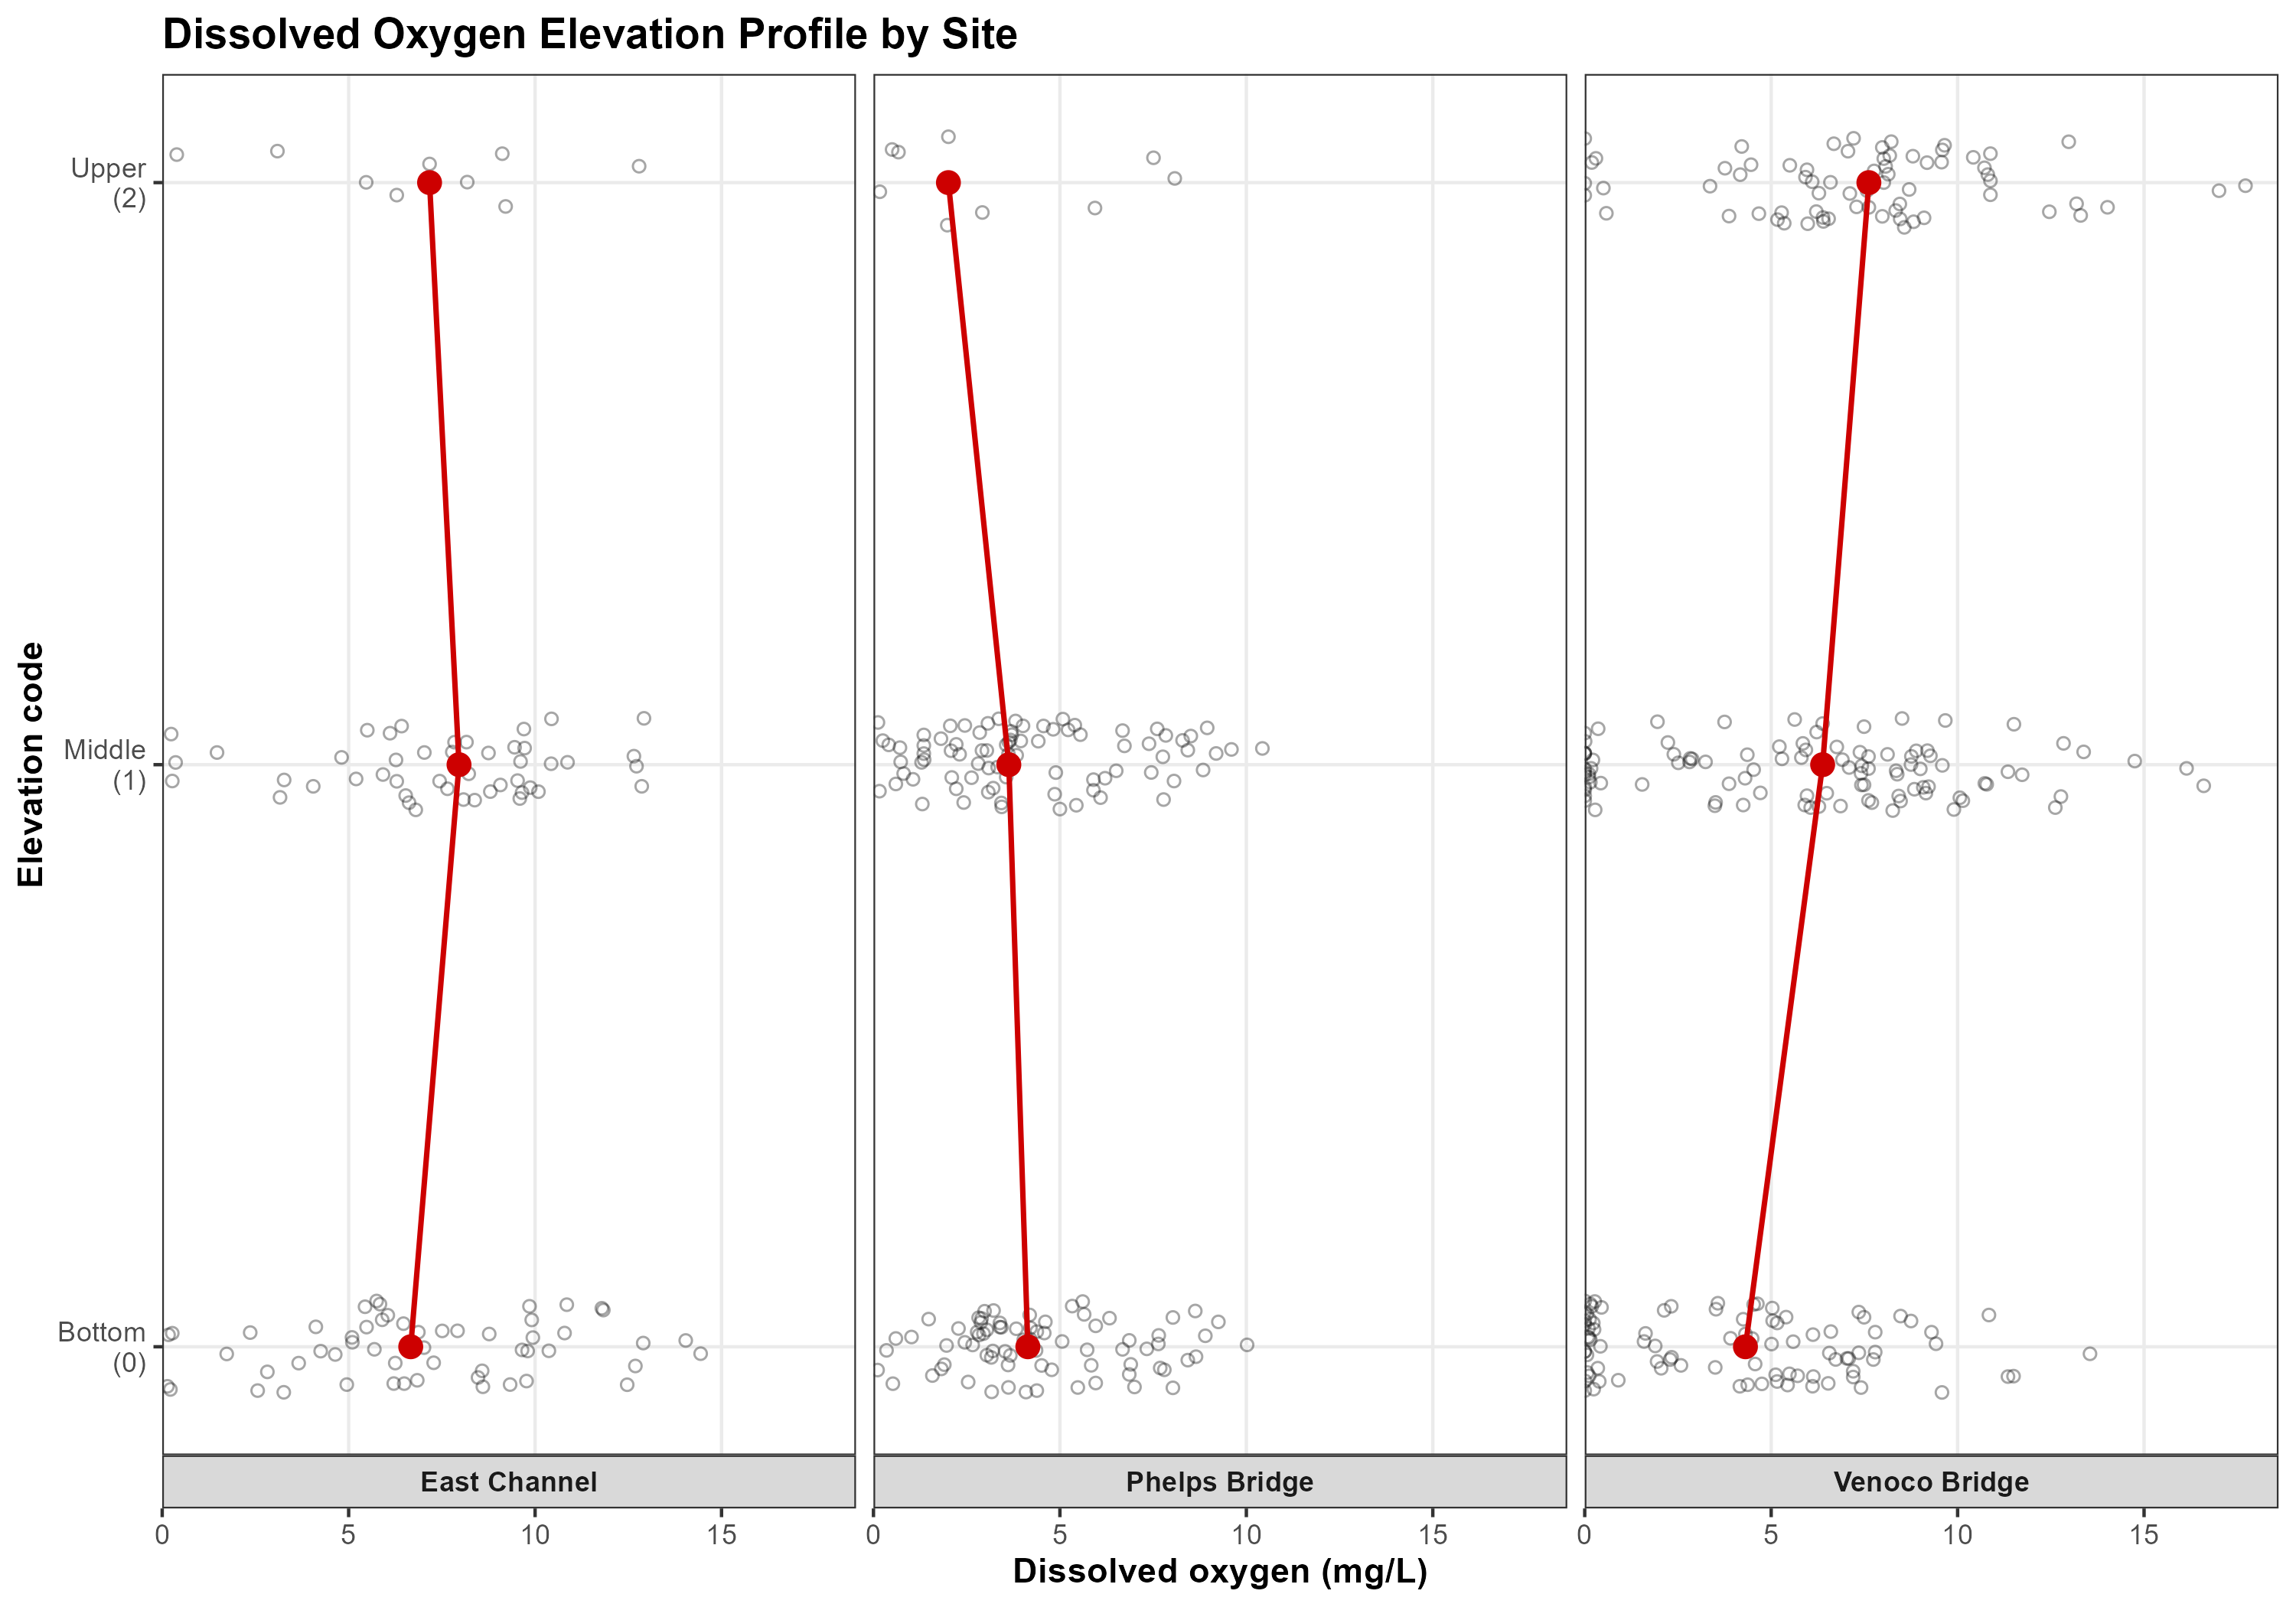
\includegraphics[width=0.85\linewidth,height=\textheight,keepaspectratio]{../images/do_elevation_profile_by_site.png}

}

\caption{\label{fig-do-elevation-profile}Dissolved oxygen elevation
profiles by site. Points show individual dissolved oxygen observations,
red points show median values, and red lines connect median values
across elevation codes.}

\end{figure}%

Figure~\ref{fig-do-elevation-profile} shows the median dissolved oxygen
elevation profile for each site. Venoco Bridge had the strongest
bottom-to-upper increase in median dissolved oxygen, while East Channel
and Phelps Bridge showed smaller or less consistent elevation-code
patterns.

Within-site Kruskal-Wallis tests showed no significant dissolved oxygen
difference across elevation codes at East Channel, \(\chi^2\) = 1.11, df
= 2, p = 0.574. Phelps Bridge also did not show a significant difference
across elevation codes, \(\chi^2\) = 3.02, df = 2, p = 0.221. Venoco
Bridge showed a significant difference across elevation codes,
\(\chi^2\) = 28.64, df = 2, p \textless{} 0.001.

Because Venoco Bridge had a significant Kruskal-Wallis result, Dunn's
post-hoc tests were used to compare elevation-code pairs at that site.
All three elevation-code pairs were significantly different after
adjustment: bottom and middle, bottom and upper, and middle and upper.
The effect size for the Venoco Bridge elevation-code comparison was
\(\eta^2_H\) = 0.105, which was classified as moderate.

\begin{figure}[H]

\centering{

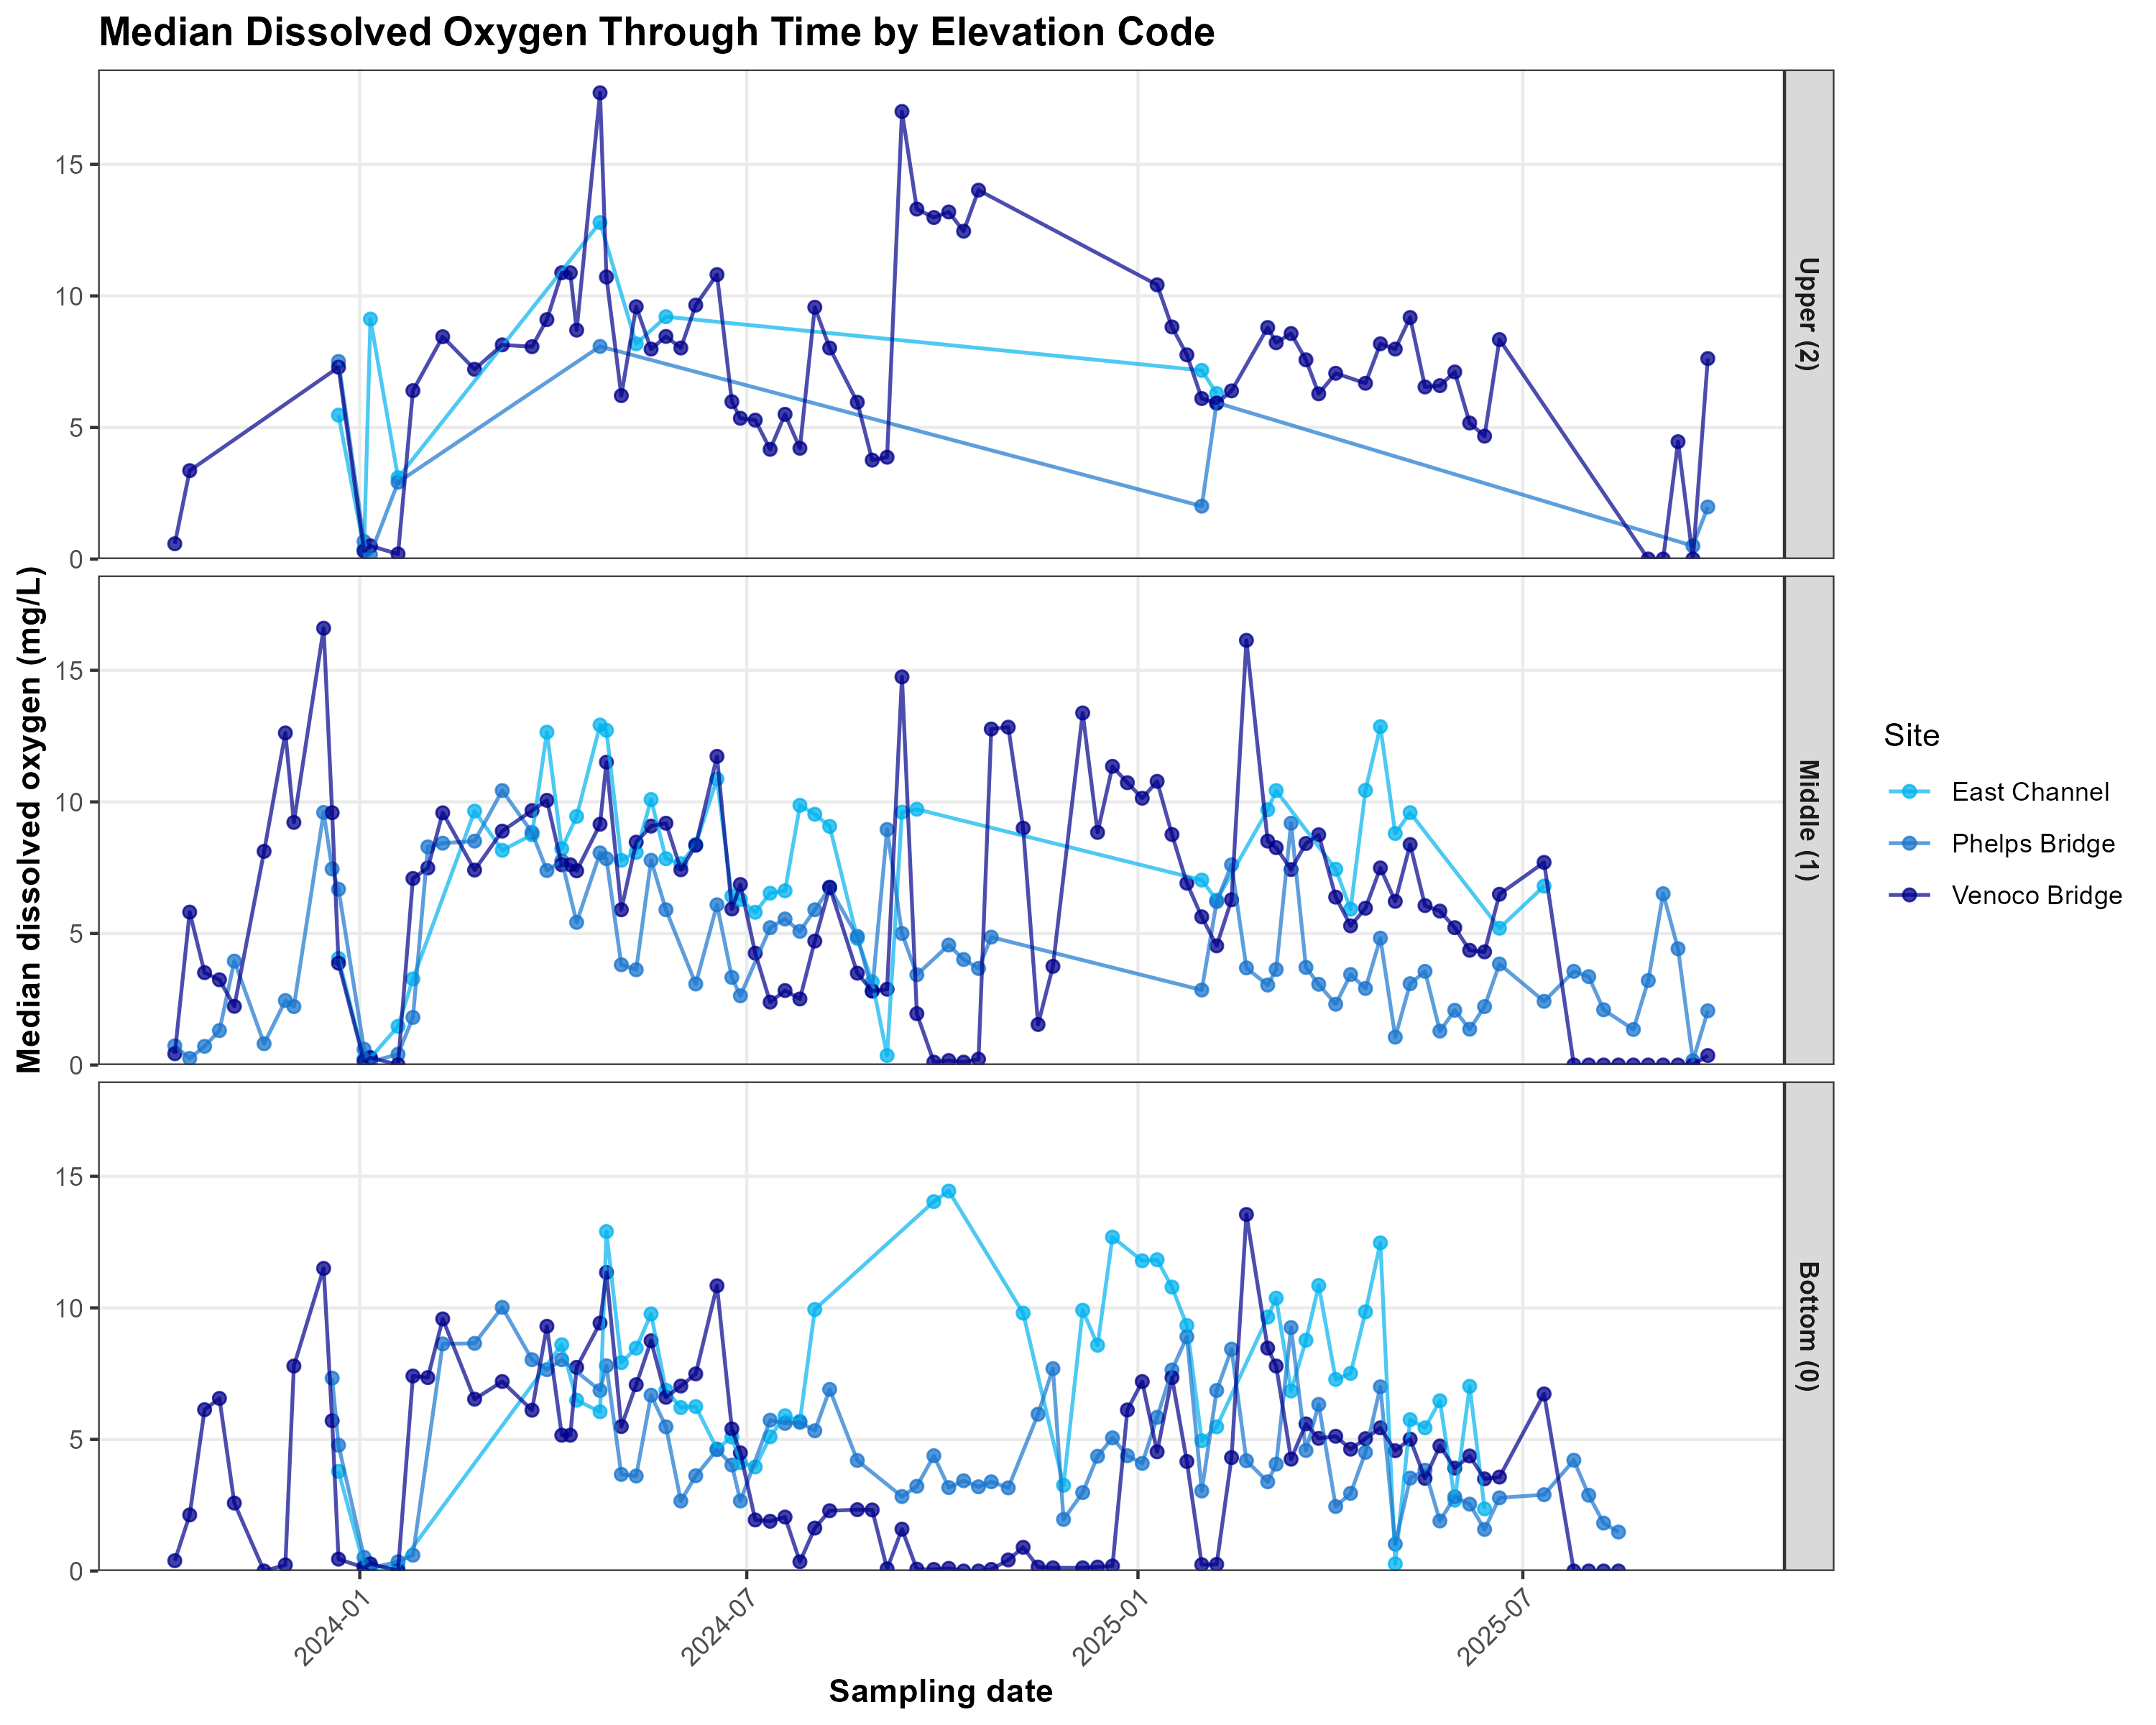
\includegraphics[width=0.9\linewidth,height=\textheight,keepaspectratio]{../images/median_do_through_time_by_elevation.png}

}

\caption{\label{fig-do-through-time}Median dissolved oxygen through time
by elevation code and site. Points represent median dissolved oxygen for
each sampling date and site, and lines connect values within each site.}

\end{figure}%

Figure~\ref{fig-do-through-time} presents median dissolved oxygen
through time by elevation code and site. Median dissolved oxygen values
varied across sampling dates, sites, and elevation codes during the 2024
and 2025 water years.

Overall, dissolved oxygen differed across East Channel, Phelps Bridge,
and Venoco Bridge. Dissolved oxygen differences across elevation codes
were statistically significant at Venoco Bridge, but not at East Channel
or Phelps Bridge.

\section{Discussion}\label{discussion}

The results show that dissolved oxygen conditions differed across the
three NCOS sites. East Channel had the highest median dissolved oxygen,
Phelps Bridge had the lowest median dissolved oxygen, and Venoco Bridge
had the widest range of values (Figure~\ref{fig-do-across-sites}).
Dissolved oxygen also differed by elevation code at Venoco Bridge, where
median dissolved oxygen was lower at the bottom and higher at the middle
and upper measurement positions (Figure~\ref{fig-do-stratification};
Figure~\ref{fig-do-elevation-profile}). East Channel and Phelps Bridge
did not show significant dissolved oxygen differences across elevation
codes.

These results show where dissolved oxygen differed, but they do not
identify one clear cause. The three sites are in different parts of
NCOS, and they likely differ in water movement, vegetation, depth,
salinity, and connection to other parts of the slough. Any of these
factors could affect dissolved oxygen, but this analysis did not
directly test which factor was most important. Because of that, the
results should be interpreted as evidence of site-level and
elevation-code differences in dissolved oxygen, not as proof of what
caused those differences.

The site-level pattern is useful because dissolved oxygen often varies
within coastal wetland and lagoon systems. In the Carmel River Lagoon,
dissolved oxygen varied across different branches of the estuary as
hydrologic conditions and mouth state changed (Dawson et al. 2023).
Water quality in intermittently closed and open lagoons can also change
with ocean connection, opening events, and mixing (Mayjor et al. 2023).
These studies support the idea that different parts of the same coastal
wetland system can have different dissolved oxygen conditions.

The Venoco Bridge pattern also fits with research on vertical dissolved
oxygen differences in shallow lagoons and estuaries. When water is not
fully mixed, bottom water can become lower in oxygen while upper water
remains more oxygenated (Gale et al. 2006, Nezlin et al. 2009). In this
project, Venoco Bridge showed the clearest bottom-to-upper difference in
dissolved oxygen. This could reflect stronger stratification at that
site, but additional data on depth, salinity, water movement, and timing
would be needed to confirm that.

Dissolved oxygen matters because it is connected to aquatic habitat
conditions. Low dissolved oxygen can reduce habitat suitability for fish
and other nekton in marsh and wetland systems (Smith and Able 2003,
Clark et al. 2025). Oxygen conditions can also affect decomposition
pathways and where invertebrates are active in shallow wetlands (Lee et
al. 2017). This project did not measure fish, invertebrate responses, or
decomposition, so it cannot make conclusions about biological effects.
It can only show that dissolved oxygen conditions differed across the
study sites and measurement positions.

Other variables would explain the dissolved oxygen patterns in this
dataset. Temperature is relevant because warmer water holds less oxygen
and can also increase biological respiration. Salinity is relevant
because salinity differences can affect water density and mixing. Both
temperature and salinity were included in the YSI water quality data.
Weather variables, such as air temperature and precipitation, were
included in the NOAA dataset and can provide context for changes across
sampling dates. Other variables, such as water depth, vegetation, algae,
wind, turbidity, and connection to the ocean or slough mouth, may also
influence dissolved oxygen, but they would require additional field
observations or more detailed site data.

One limitation of this analysis is that the dataset used repeated
monitoring observations rather than continuous dissolved oxygen sensor
data. This means the analysis shows patterns across the available
sampling dates, sites, and elevation codes, but it does not capture all
short-term changes within a day. Dissolved oxygen in shallow wetlands
can change over daily cycles because of light, photosynthesis,
respiration, and temperature (Smith and Able 2003, Reeder 2011,
Koop-Jakobsen and Gutbrod 2019). Time of day and sampling conditions
could therefore affect the dissolved oxygen values measured during
monitoring.

Collecting dissolved oxygen data in a restored wetland also has
practical challenges. Wetland conditions can change with water level,
weather, vegetation, mud, and site access. Measurements also depend on
reaching similar locations and water-column positions across sampling
dates. These challenges matter because small differences in sampling
depth, timing, or field conditions could affect dissolved oxygen values.
The NCOS monitoring report provides the broader restoration and
monitoring context for interpreting these water quality patterns at the
site (Rickard 2024).

In addition, the elevation-code comparisons pooled measurements
collected on many different dates, so the within-site differences
reflect both vertical position and the conditions on each sampling date,
rather than stratification measured at a single moment. Comparing bottom
and upper DO from the same sampling event would give a more direct
measure of stratification.

Future work could build on this analysis by comparing dissolved oxygen
more directly with temperature, salinity, water depth, season, and time
of day. Continuous dissolved oxygen sensors would also help show daily
oxygen cycles that repeated monitoring may miss. These additions would
make it easier to determine whether the patterns observed here are
related to mixing, stratification, seasonal change, or other site
conditions.

\section{Conclusion}\label{conclusion}

Dissolved oxygen differed across East Channel, Phelps Bridge, and Venoco
Bridge during the 2024 and 2025 water years. East Channel had the
highest median dissolved oxygen, Phelps Bridge had the lowest median
dissolved oxygen, and Venoco Bridge had the widest range of values.

Dissolved oxygen differences across elevation-code positions were
strongest at Venoco Bridge. At this site, median dissolved oxygen was
lower at the bottom and higher at the middle and upper measurement
positions. East Channel and Phelps Bridge did not show significant
dissolved oxygen differences across elevation codes.

These findings show that dissolved oxygen conditions were not the same
across all parts of NCOS. Continued monitoring, especially with added
attention to temperature, salinity, water depth, season, and time of
day, could help explain what drives these differences across the
restored wetland.

\section*{References}\label{references}
\addcontentsline{toc}{section}{References}

\protect\phantomsection\label{refs}
\begin{CSLReferences}{1}{0}
\bibitem[\citeproctext]{ref-clark2025}
Clark, A., W. T. Ellis, A. R. Rodriguez, and R. Baker. 2025.
\href{https://doi.org/10.1007/s12237-025-01525-0}{Dissolved oxygen may
limit the suitability of salt marsh as nekton habitat}. Estuaries and
Coasts 48.

\bibitem[\citeproctext]{ref-dawson2023}
Dawson, J., M. M. Orescanin, R. Clark, and K. O'Connor. 2023.
\href{https://doi.org/10.1016/j.ecss.2023.108241}{Spatiotemporal
variability of dissolved oxygen in response to morphological state in a
central california coast bar-built estuary}. Estuarine, Coastal and
Shelf Science 282:108241.

\bibitem[\citeproctext]{ref-gale2006}
Gale, E., C. Pattiaratchi, and R. Ranasinghe. 2006.
\href{https://doi.org/10.1016/j.ecss.2006.04.013}{Vertical mixing
processes in intermittently closed and open lakes and lagoons, and the
dissolved oxygen response}. Estuarine, Coastal and Shelf Science
69:205--216.

\bibitem[\citeproctext]{ref-koopjakobsen2019}
Koop-Jakobsen, K., and M. S. Gutbrod. 2019.
\href{https://doi.org/10.3389/fenvs.2019.00137}{Shallow salt marsh tidal
ponds: An environment with extreme oxygen dynamics}. Frontiers in
Environmental Science 7:137.

\bibitem[\citeproctext]{ref-vanderlee2017}
Lee, G. H. van der, M. H. S. Kraak, R. C. M. Verdonschot, J. A. Vonk,
and P. F. M. Verdonschot. 2017.
\href{https://doi.org/10.1038/s41598-017-15432-3}{Oxygen drives
benthic-pelagic decomposition pathways in shallow wetlands}. Scientific
Reports 7.

\bibitem[\citeproctext]{ref-mayjor2023}
Mayjor, M., A. J. Reichelt-Brushett, H. A. Malcolm, and A. Page. 2023.
\href{https://doi.org/10.1016/j.ecss.2022.108208}{Water quality
fluctuations in small intermittently closed and open lakes and lagoons
(ICOLLs) after natural and artificial openings}. Estuarine, Coastal and
Shelf Science 281:108208.

\bibitem[\citeproctext]{ref-nezlin2009}
Nezlin, N. P., K. Kamer, J. Hyde, and E. D. Stein. 2009.
\href{https://doi.org/10.1016/j.ecss.2009.01.004}{Dissolved oxygen
dynamics in a eutrophic estuary, upper newport bay, california}.
Estuarine, Coastal and Shelf Science 82:139--151.

\bibitem[\citeproctext]{ref-reeder2011}
Reeder, B. C. 2011.
\href{https://doi.org/10.1016/j.ecolind.2011.04.006}{Assessing
constructed wetland functional success using diel changes in dissolved
oxygen, pH, and temperature in submerged, emergent, and open-water
habitats in the beaver creek wetlands complex, kentucky (USA)}.
Ecological Indicators 11:1772--1788.

\bibitem[\citeproctext]{ref-rickard2024}
Rickard, A. 2024. \href{https://escholarship.org/uc/item/16p046mb}{North
campus open space restoration project monitoring report: Year 7,
december 2024}. UC Santa Barbara: Cheadle Center for Biodiversity and
Ecological Restoration.

\bibitem[\citeproctext]{ref-smith2003}
Smith, K. J., and K. W. Able. 2003.
\href{https://doi.org/10.3354/meps258223}{Dissolved oxygen dynamics in
salt marsh pools and its potential impacts on fish assemblages}. Marine
Ecology Progress Series 258:223--232.

\end{CSLReferences}




\end{document}
